\section{Results}
\label{sec:results}
All results are for the octahedron of \cref{sec:inertia} simulated with the spring engines, unless stated otherwise.
The figures and numbers in this section come from \code{plot_results.py} and \code{plot_flip_time.py} in \code{src/sim/}.

\subsection{Stable rotation about the major and minor axes}
\label{sec:res-stable}
To compare the three axes directly, we spun the body at \SI{1}{rad/s} about each principal axis in turn, tilted by $\varepsilon=0.01$ toward the next axis, and followed it for \SI{100}{s} with the Python engine ($\Delta t=\SI{1}{ms}$, $k=\SI{e5}{N/m}$).
\Cref{fig:stable} shows the angle between the spin axis of the body and the fixed angular momentum.
About the axes of largest and smallest moment this angle only oscillates, between \ang{0.2} and \ang{0.44} about $x$ and between \ang{1.49} and \ang{1.65} about $z$, and does not grow over the whole run.
About the middle axis the same small tilt, initially \ang{0.29}, grows until the axis has turned over completely to \ang{180}, and then returns, about every \SI{48}{s}.

\begin{figure}[htb]
    \centering
    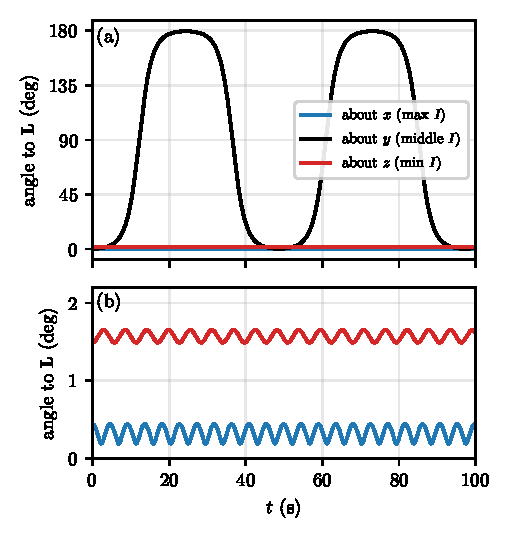
\includegraphics[width=\linewidth]{Images/stable_axes.pdf}
    \caption{Angle between the spin axis of the body and $\vb{L}$ for spins about each principal axis with the same small tilt. (a) All three runs: only rotation about the middle axis $y$ turns over. (b) Zoom on the runs about $x$ and $z$, where the angle stays bounded.}
    \label{fig:stable}
\end{figure}

\subsection{Rotation about the intermediate axis}
\label{sec:res-flip}
\begin{sloppypar} % long inline vector would otherwise stick out of the column
The main run spins the body about its middle axis with the Rust engine ($\Delta t=\SI{e-5}{s}$, $k=\SI{e5}{N/m}$, \SI{100}{s}); it is shown in \cref{fig:vis-omega,fig:vis-polhode}.
The body flips three times, each flip being a sign change of the component of $\vb{L}$ along the middle axis.
To test these times we solved Euler's equations (\cref{eq:euler}) for an ideal rigid body with SciPy's \code{solve_ivp} \cite{scipy} at a relative tolerance of $10^{-12}$, starting from the same angular velocity as the simulation, $\Omega_k=L_k(0)/I_k$, which gives $\vb*{\Omega}_0\approx(0.0015,1.0001,0)$\,\si{rad/s}.
The two agree to within one output frame, $\tfrac{1}{60}$\,s (\cref{tab:flips}), and the flips repeat every \SI{31.2}{s}.
Over the run the simulated $\vb{L}$ stays on the predicted polhode: $2E/L^2$ changes by less than $10^{-5}$ of its value, and $\abs{\vb{L}}$ by $1.4\times10^{-4}$, the latter mostly from the finite-difference velocities.
\end{sloppypar}

\begin{table}[htb]
    \centering
    \caption{Flip times for spin about the middle axis.}
    \label{tab:flips}
    \small
    \begin{tabular}{@{}lccc@{}}
        \toprule
                                      & 1st (s) & 2nd (s) & 3rd (s) \\
        \midrule
        Spring engine          & 15.60   & 46.82   & 78.03 \\
        Rigid body (Euler) & 15.61   & 46.82   & 78.03 \\
        \bottomrule
    \end{tabular}
\end{table}

\subsection{Flip time versus perturbation size}
\label{sec:res-fliptime}
\begin{sloppypar} % numbers with units would otherwise stick out of the column
\Cref{fig:flip-time} shows the time to the first flip for 500 initial tilts $\varepsilon$ between $2\times10^{-7}$ and $10^{-4}$, computed with the Rust engine ($\Delta t=\SI{1}{ms}$) for several spring stiffnesses, together with the rigid-body solution.
The flip time grows without bound as $\varepsilon\to0$, but only slowly: halving the tilt adds the same fixed amount of time.
Fitting $t_{\text{flip}}=\lambda^{-1}\ln(1/\varepsilon)+c$ to each set (\cref{tab:lambda}) confirms the logarithmic law of \cref{eq:tflip}; every fit has $R^2>0.9999996$.
For the stiffest springs the fitted growth rate, $\lambda=0.480383\pm0.000003\,\si{s^{-1}}$, matches the prediction of \cref{eq:lambda}, $\lambda=0.480384\,\si{s^{-1}}$, within its uncertainty.
Softer springs give a smaller $\lambda$ and later flips: the body stretches under its own rotation, which changes its moments of inertia.
\end{sloppypar}

\begin{figure}[htb]
    \centering
    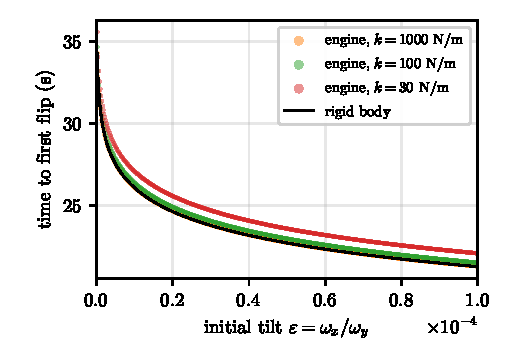
\includegraphics[width=\linewidth]{Images/flip_time.pdf}
    \caption{Time to the first flip against the initial tilt from the middle axis. Points: spring engine for three stiffnesses. Line: ideal rigid body from Euler's equations.}
    \label{fig:flip-time}
\end{figure}

\begin{table}[htb]
    \centering
    \caption{Growth rate $\lambda$ fitted to the flip times, compared with \cref{eq:lambda}.}
    \label{tab:lambda}
    \small
    \begin{tabular}{@{}lcc@{}}
        \toprule
        $k$ (N/m) & $\lambda$ (s$^{-1}$) & $\lambda/\lambda_{\text{theory}}$ \\
        \midrule
        $10^5$ & 0.48038 & 1.0000 \\
        $10^3$ & 0.47981 & 0.9988 \\
        $100$  & 0.47466 & 0.9881 \\
        $30$   & 0.46191 & 0.9615 \\
        \midrule
        Theory & 0.48038 & \\
        \bottomrule
    \end{tabular}
\end{table}

\subsection{Dissipation: relaxation to the major axis}
\label{sec:res-major}
The model and the expected outcome are described in \cref{sec:extension}; \cref{fig:dissipation} shows the damped run of the Rust engine.
At the start $\vb{L}$ is \ang{14.6} from the minimum axis $z$.
Over the first few hundred seconds the body wobbles away from $z$ and settles on the maximum axis $x$: by the end $\vb{L}$ is within \ang{0.7} of $x$.
Meanwhile $\abs{\vb{L}}$ stays constant to $5\times10^{-5}$, as it should for central damping forces.

\begin{sloppypar} % numbers with units would otherwise stick out of the column
The kinetic energy first drops quickly from \SI{5.13}{J} to about \SI{3.9}{J}, because the springs start at their rest length: the spinning body first expands, storing part of the energy in the springs, and the fast oscillation this starts is damped away at once.
After that it decays steadily and levels off at \SI{1.948}{J}.
This final value equals $L^2/2I_x=\SI{1.948}{J}$ when $I_x$ is computed from the actual, stretched shape of the body at the end ($I_x=\SI{27.4}{kg.m^2}$ instead of 26 at rest), so the body ends in steady rotation about $x$ at $\Omega_x=\SI{0.377}{rad/s}$.
The estimates of \cref{sec:extension}, \SI{2.05}{J} and \SI{0.40}{rad/s}, used the moment at rest, and the difference is exactly this stretching.
\end{sloppypar}

\begin{figure}[htb]
    \centering
    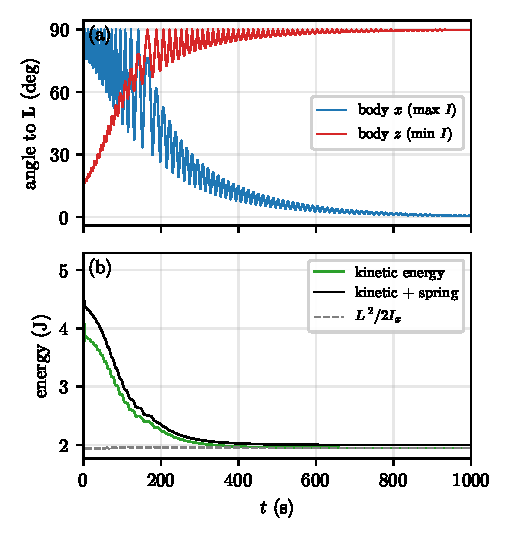
\includegraphics[width=\linewidth]{Images/dissipation.pdf}
    \caption{Damped body started near its minimum axis. (a) Angle between $\vb{L}$ and the body axes $x$ (max $I$) and $z$ (min $I$): the spin moves from $z$ to $x$. (b) Kinetic energy, kinetic plus spring energy, and the lowest energy possible at this $L$, $L^2/2I_x$, computed from the current shape of the body.}
    \label{fig:dissipation}
\end{figure}
